\documentclass[12pt]{article}
\usepackage[pdfborder={0 0 0.5 [3 2]}]{hyperref}%
\usepackage[left=1in,right=1in,top=1in,bottom=1in]{geometry}%
\usepackage[shortalphabetic]{amsrefs}%
\usepackage{amsmath}
\usepackage{enumerate}
\usepackage{enumitem}
\usepackage{amssymb}                
\usepackage{amsmath}                
\usepackage{amsfonts}
\usepackage{amsthm}
\usepackage{bbm}
\usepackage[table,xcdraw]{xcolor}
\usepackage{tikz}
\usepackage{float}
\usepackage{booktabs}
\usepackage{svg}
\usepackage{mathtools}
\usepackage{cool}
\usepackage{url}
\usepackage{graphicx,epsfig}
\usepackage{framed}
\usepackage{hyperref}  

\usetikzlibrary{automata,arrows,positioning,calc}
\DeclarePairedDelimiter\abs{\lvert}{\rvert}%
\DeclarePairedDelimiter\norm{\lVert}{\rVert}%
\DeclarePairedDelimiter\ceil{\lceil}{\rceil}
\DeclarePairedDelimiter\floor{\lfloor}{\rfloor}

\makeatletter
\renewcommand*\env@matrix[1][*\c@MaxMatrixCols c]{%
  \hskip -\arraycolsep
  \let\@ifnextchar\new@ifnextchar
  \array{#1}}
\makeatother

\newtheorem{theorem}{Theorem}[section]
\newtheorem{corollary}{Corollary}[theorem]
\newtheorem{proposition}[theorem]{Proposition}
\newtheorem{lemma}[theorem]{Lemma}

\theoremstyle{definition}
\newtheorem{definition}[theorem]{Definition}
\newtheorem{exercise}{Exercise}%
\newtheorem{problem}[exercise]{Problem}%
\newtheorem*{example}{Example}

\theoremstyle{remark}
\newtheorem*{question}{Question}
\newtheorem*{observation}{Observation}
\newtheorem*{remark}{Remark}

\graphicspath{ {images/} }

\setlength{\parindent}{0cm}
\renewcommand{\vec}[1]{\ensuremath{\mathbf{#1}}}

\def\noi{\noindent}
\def\T{{\mathbb T}}
\def\R{{\mathbb R}}
\def\N{{\mathbb N}}
\def\C{{\mathbb C}}
\def\Z{{\mathbb Z}}
\def\P{{\mathbb P}}
\def\E{{\mathbb E}}
\def\Q{\mathbb{Q}}
\def\ind{{\mathbb I}}

\def\cale{{\mathcal E}}
\def\cals{{\mathcal S}}
\def\calc{{\mathcal C}}
\def\caln{{\mathcal N}}
\def\calb{{\mathcal B}}
\def\calg{{\cal G}}

\def\ds{\displaystyle}
\def\ra{\rightarrow}
\newcommand{\conv}{\mbox{\rm conv}}
\newcommand{\spaan}{\mbox{\rm span}}
\newcommand{\deet}{\mbox{\rm det}}
\newcommand{\aff}{\mbox{\rm aff}}
\newcommand{\cl}{\mbox{\rm cl}}
\newcommand{\dimm}{\mbox{\rm dim}}
\newcommand{\sm}{\setminus}
\def\ci{\perp\!\!\!\perp}

\newcommand{\ink}{\rule{.5\baselineskip}{.55\baselineskip}}

\begin{document}

\setcounter{section}{1}
\section{Discrete Random Variables}

\subsection{Random Variables}
A \emph{random variable} is a real-valued function on a sample space\footnote{It's not really a variable at all, but we are stuck with the terminology.}. A random variable generally is a quantity we wish to measure; the output of the random variable depends on which element of the sample space is chosen. In this section, we will look at discrete random variables.

\begin{framed}
A \emph{discrete} random variable $Y$ is a random variable which can only take on a finite or countable set of distinct values.
\end{framed}

Here are some examples of discrete random variables:
\begin{enumerate}
\item The number of voters in Rhode Island who prefer Hillary Clinton.
\item The number of defective lightbulbs out of a shipment of 1000 lightbulbs.
\item The number of times I play a slot machine in Las Vegas until I win.
\end{enumerate}

We will use the following simple example to illustrate features of discrete random variables.

\begin{example}Let $\cals$ be the sample space representing the flip of two fair coins. Let $Y$ be the number of heads flipped. Then $Y$ is a discrete random variable, since it can only have the values 0, 1, or 2. We can illustrate it graphically below.
\begin{figure}[H]
\centering
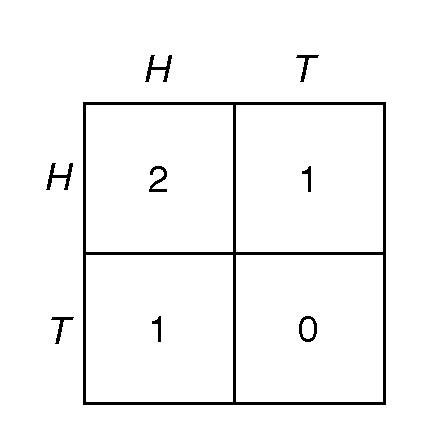
\includegraphics[width=3cm]{numberofheads.eps}
\end{figure}
\end{example}

Uppercase letters, such as $Y$, are used to designate random variables. We use lowercase letters, such as $y$, to designate a value that a random variable can take. The expression $(Y = y)$ is shorthand for the set of all points in our sample space $\cals$ for which the random variable $Y$ outputs the value $y$. Since $(Y = y)$ is a subset of $\cals$, it is an event in our sample space. In the two-coin-toss problem, for example, the possible values of $Y$ are 0, 1, and 2, so we have:
\begin{itemize}[noitemsep]
\item $(Y = 0) = \{ (T, T) \}$
\item $(Y = 1) = \{ (H, T), (T, H) \}$
\item $(Y = 2) = \{ (H, H) \}$
\end{itemize}

Since $(Y = y)$ is an event in our sample space, we can talk about its probabiltiy, i.e. $\P(Y = y)$. In fact, the point of random variables is to do just this! 

\begin{framed}
  \emph{Probability of a discrete random variable }\\
  \rule{\dimexpr\linewidth-2\fboxsep-2\fboxrule}{.1pt} \\
  The probability that a discrete random variable $Y$ takes the value $y$, denoted $\P(Y = y)$, or $p(y)$ for short, is the probability of the event $(Y = y)$, the set of all points in the sample space $\cals$ which output the value $y$. \\

  $\P(Y = y)$ is the sum of the probabilities of all the simple events in $\cals$ which are assigned the value $y$ by the random variable $Y$.
\end{framed}

Back to our two-coin-toss problem, let's look at the probabilties of the random variable $Y$. For convenience, here is a picture of the sample space probabilities next to a graphical representation of $Y$. Since we are using the discrete uniform distribution for coin tosses, each simple event in our sample space has probability 1/4.
\begin{figure}[H]
\centering
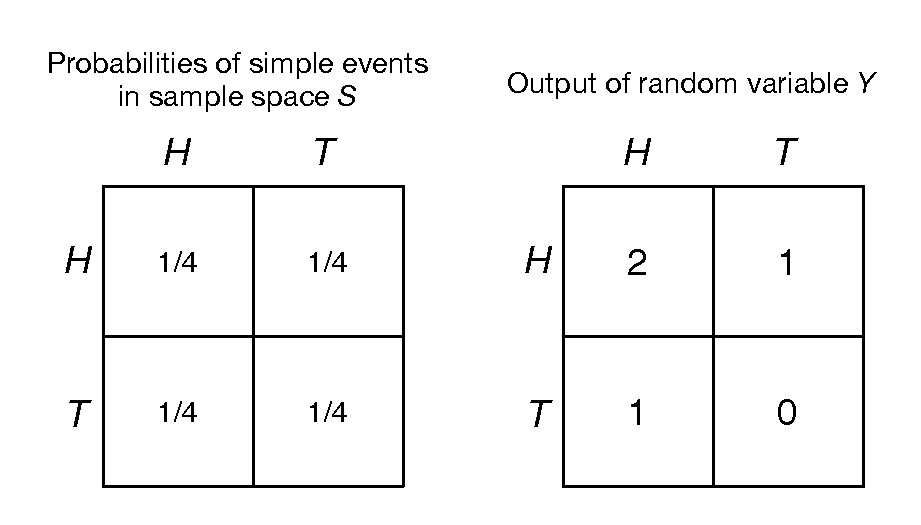
\includegraphics[width=8cm]{numberofheads2.eps}
\end{figure}

Using the rule above, we can compute the following probabilties for $Y$ by adding up the probabilities of the underlying simple events. In this case, since we are using the discrete uniform distribution, we could also just count the number of simple events which lead to each output of $Y$ and divide by 4, the size of the sample space.
\begin{itemize}[noitemsep]
\item $\P(Y = 0) = 1/4$
\item $\P(Y = 1) = 1/4 + 1/4 = 1/2$
\item $\P(Y = 2) = 1/4$
\end{itemize}

\begin{framed}
  \emph{Probability mass function }\\
  \rule{\dimexpr\linewidth-2\fboxsep-2\fboxrule}{.1pt} \\
  The \emph{probablity mass function (pmf)} is a function which gives the probabiltiy that a discrete random variable $Y$ is exactly equal to a value $y$. The pmf can be represented as a function, table, or graph which gives the values $p(y) = \P(Y = y)$ for all possible values $y$ which $Y$ can take.
\end{framed}

In the two-coin-flip example, we can represent the pmf of $Y$ in a table:
\begin{figure}[H]
\centering
\begin{tabular}{l@{\hskip 2cm}l}
\toprule
$y$ & $p(y)$\\
\midrule
0 & 1/4\\
1 & 1/2\\
2 & 1/4\\
\bottomrule
\end{tabular}
\end{figure}

We can also represent the pmf graphically as a histogram\footnote{I will undoubtedly lose some of my math street cred if I admit to using Microsoft Excel for these histograms, but in some cases it really is the easiest tool to use.}.
\begin{figure}[H]
\centering
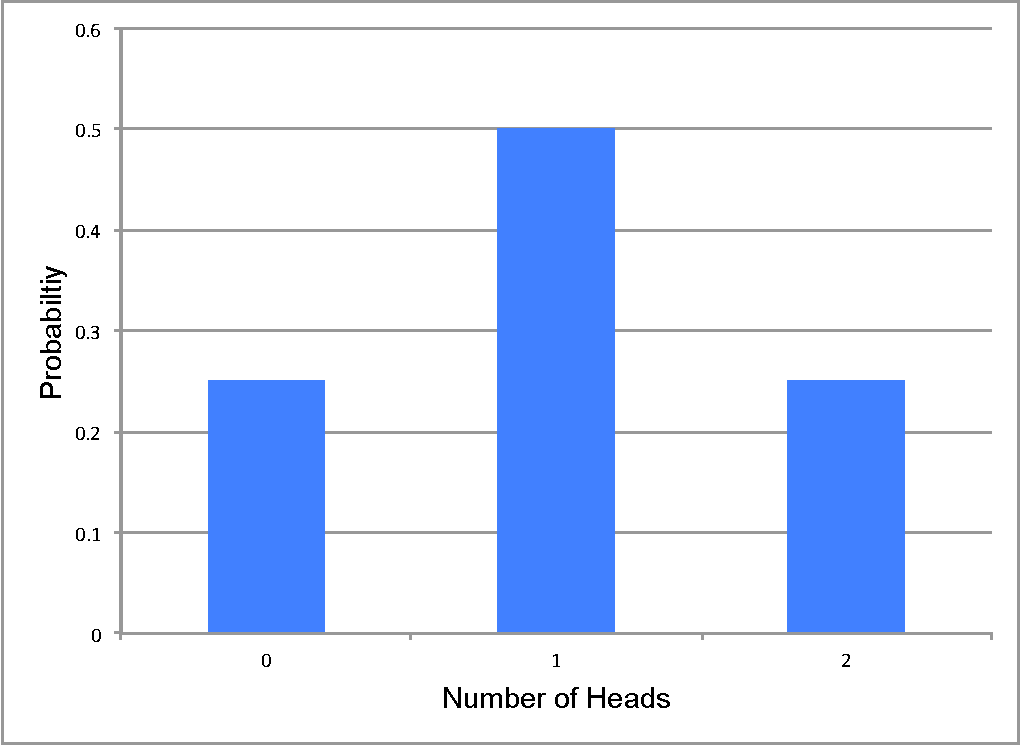
\includegraphics[width=5cm]{2coinshisto}
\end{figure}


A discrete random variable induces a probability distribution on the sample space of all possible values the random variable can take. This is a different sample space from the original sample space. Back to our two-coin-flip example, the random variable $Y$ induces a probability distribution on a new sample space $\mathcal{T} = \{0, 1, 2\}$. The probabilities of the sample points in $\mathcal{T}$ are the probabilties $p(y)$ for $y = 0, 1, 2$. We can illustrate this new sample space in a picture.

\begin{figure}[H]
\centering
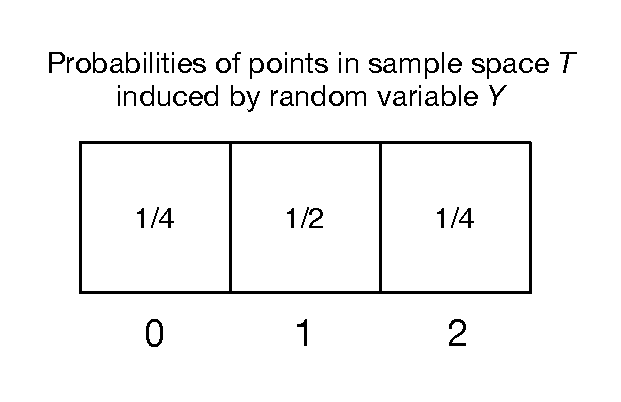
\includegraphics[width=5cm]{induced1.eps}
\end{figure}

Often (as we shall see), we care much more about the sample space induced by a random variable than the underlying sample space. Since a discrete random variable induces a probability distribution, the following must be true.

\begin{framed}
For any discrete random variable $Y$:
\begin{align*}
0 \leq p(y) &\leq 1 \:\text{ for all }y \\
\sum_{\text{all } y} p(y) &= 1
\end{align*}
where $p(y) = \P(Y = y)$. Since we have a discrete sample space, the sum is finite or countable.
\end{framed}

Let's look at two more examples, this time involving the rolls of two six-sided dice.

\begin{example}Let $\cals$ be the sample space representing the rolls of two six-sided dice. Consider the following two random variables:
\begin{enumerate}
\item $X$ = the sum of the two dice
\item $Y$ = the larger of the two die rolls (if they are the same, then it's just equal to both die rolls)
\end{enumerate} 
Let's look at these random variables graphically.
\begin{figure}[H]
\centering
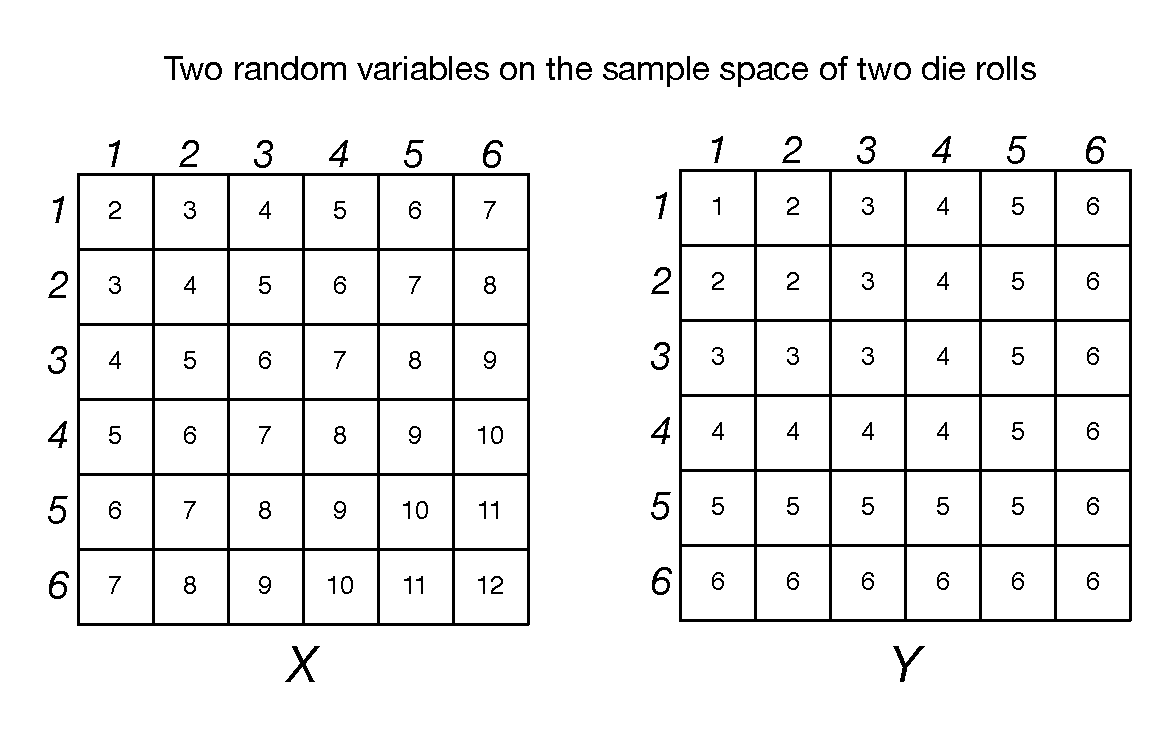
\includegraphics[width=10cm]{2dicervs.eps}
\end{figure}

The random variable $X$ induces a probability distribution on the set of integers $\{2, 3, 4, \dots, 12\}$, and the random variable $Y$ induces a probability distribution on the set of integers $\{1, 2, 3, 4, 5, 6\}$. Let's look at the pmfs of both random variables using histograms.

\begin{figure}[H]
\centering
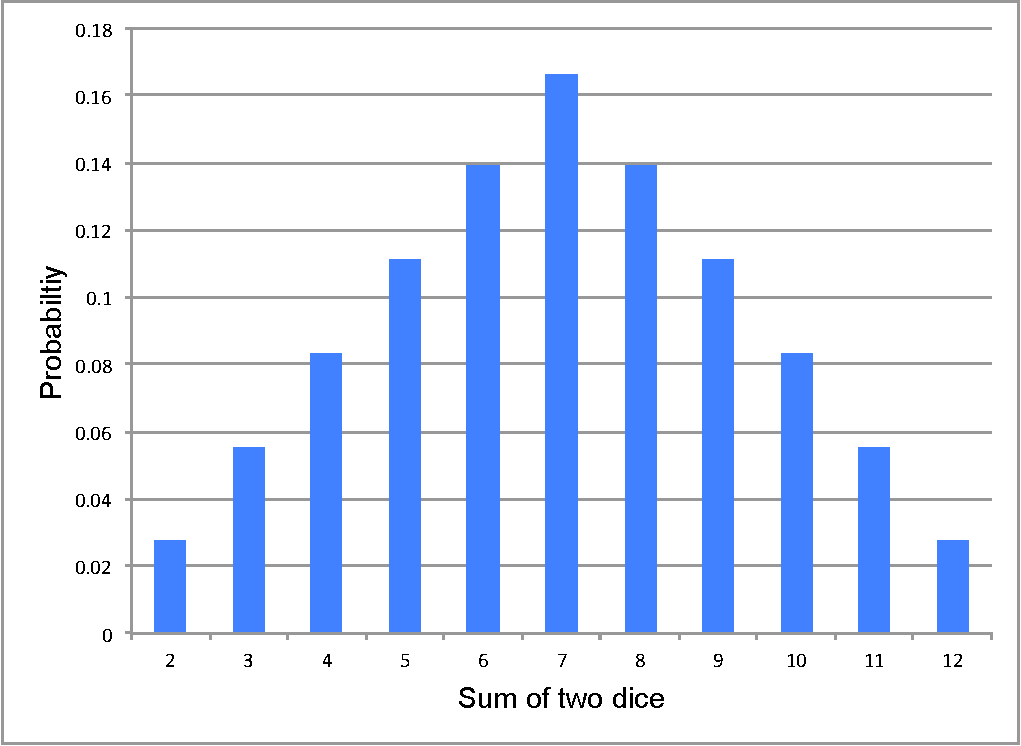
\includegraphics[width=7cm]{sumoftwodice.pdf}
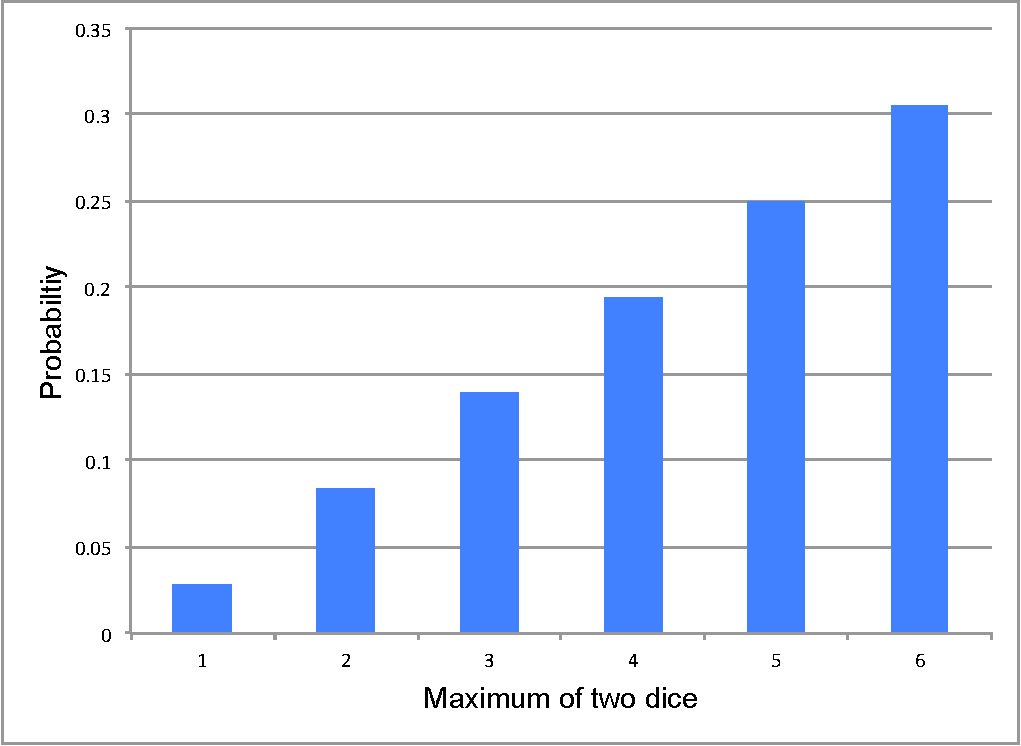
\includegraphics[width=7cm]{maxoftwodice.pdf}
\end{figure}
Both of these distributions are nonuniform, even though the underlying distribution of the two dice is uniform. The first distribution, that of the random variable $X$, is a familiar one to afficionados of board games such at Settlers of Catan and Monopoly. We can also write the pmfs in table form. For the random variable $Y$, we have:
\begin{figure}[H]
\centering
\begin{tabular}{l@{\hskip 2cm}l}
\toprule
$y$ & $p(y)$\\
\midrule
1 & 1/36\\
2 & 3/36\\
3 & 5/36\\
4 & 7/36\\
5 & 9/36\\
6 & 11/36\\
\bottomrule
\end{tabular}
\end{figure}
The pmf for $X$ can be expressed similarly.
\end{example}

\subsection{Expected Value}
Given a discrete random variable, we can definite it's mean, or expected value. 

\begin{framed}
  \emph{Expected value of a random variable}\\
  \rule{\dimexpr\linewidth-2\fboxsep-2\fboxrule}{.1pt} \\
For a discrete random variable $Y$ with probability function $p(y)$, the \emph{expected value} or \emph{mean} is defined to be
\[
\E(Y) = \sum_{\text{all }y}y\:p(y)
\]
where the sum is taken over all possible values $y$ can take. We can think of the expected value as a weighted average of the values of $Y$ with each possible output $y$ weighted by its probability $p(y)$. The expected value is sometimes written as $\mu$ (for mean)
\end{framed}

Here is one interpretation of the expected value of a random variable. Think of a random variable $Y$ as an observation from an experiment. Suppose we perform the experiment $n$ times, and observe $n$ values of $Y$, which we shall designate $y_1, y_2, \dots, y_n$. Then for large $n$,
\[
\frac{y_1 + y_2 + \cdots + y_n}{n} \approx \E(Y)
\]
where the approximation ``gets better'' as $n$ gets larger, i.e. as we perform more experiments. The quantity on the left hand side is known as the \emph{empirical mean} or \emph{sample mean} and looks like what we likely learned in high school (add a bunch of stuff up and divide by the number of things). The expected value is, in a sense, the limit of the empirical mean as the sample size approaches infinity. We will make this more precise later in the course, but this is a good concept to keep in mind.

\begin{example}Let $X$ represent the roll of a standard, fair six-sided die. (In this case, the underlying sample space is $\cals = \{1, 2, 3, 4, 5, 6\}$ with the discrete uniform distribution, and the random variable $X$ is the same as the sample space element selected.) Then the expected value of $X$ is:
\begin{align*}
\E(X) &= \sum_{x = 1}^6 x \P(X = x) \\
&= \sum_{x = 1}^6 x \frac{1}{6} \\
&= \frac{1}{6 } \sum_{x = 1}^6 x \\
&= \frac{21}{6} \\
&= 3.5
\end{align*}
where used the fact from the discrete uniform distribution that $\P(X = x)$ = 1/6 for all $x$. Note that the expected value of 3.5 is not a possible value of $X$, i.e. we cannot roll a 3.5 on a single die. Given our ``long term average'' interpretation, this is saying that we expect the empirical average to approach 3.5 as the number of rolls increases, not that a 3.5 is the most likely die roll.
\end{example}

\begin{example}Let $Y$ be the random variable above representing the maximum of two dice. What is the expected value of $Y$.\\

To find the expected value, we do a weighted average using the probabities in the table above.
\begin{align*}
\E(Y) &= \sum_{y = 1}^6 y \P(Y = y) \\
&= 1 \cdot \frac{1}{36} + 2 \cdot \frac{3}{36} + 3 \cdot \frac{5}{36} + 4 \cdot \frac{7}{36} + 5 \cdot \frac{9}{36} + 6 \cdot \frac{11}{36} \\
&= \frac{1 + 6 + 15 + 28 + 45 + 66}{36} \\
&= \frac{161}{36} \approx 4.47
\end{align*}
\end{example}

\subsection{Properties of Expectation}
We will discuss several properties of the expected value. The first and and one of the most important is the \emph{linearity of expectation}.

\begin{framed}
  \emph{Linearity of expectation}\\
  \rule{\dimexpr\linewidth-2\fboxsep-2\fboxrule}{.1pt} \\
Let $X$ and $Y$ be two random variables\footnote{So far we have only discussed what an expected value is in terms of discrete random variables, but this is true for all random variable.}, and let $a$ and $b$ be constants. Then
\[
\E(aX + bY) = a\E(X) + b\E(Y)
\]
This is called \emph{linearity} in reference to linear algebra, i.e. we can separate addition and pull out constants. This holds whether or not $X$ and $Y$ are independent. \\

As a corollary of this, if we have random variables $X_1, X_2, \dots, X_n$, then
\[
\E(X_1 + X_2 + \cdots + X_n) = \E(X_1) + \E(X_2) + \cdots + \E(X_n)
\]
\end{framed}

Linearity of expectation is a really nice property since it does not require the random variables to be independent. Let's do a problem to illustrate the usefulness of linearity of expectation.

\begin{example}
One evening, $n$ customers dine at a restaurant. Each gives their hat to a hat-check person at a restaurant. (These are fashionable diners!) After dinner, the hat-check person gives the hats back to the customers in a random order, i.e. each customer receives one of the hats uniformly at random. What is the expected number of customers that get their own hat back?\\

Let $X$ be the number of customers who get their own hat back. Then $X$ is a discrete random variable taking values $0, 1, \dots, n$. By the definition of expected value:
\[
\E(X) = \sum_{i = 1}^n i \:\P(X = i)
\]
At this point, we have a mess! We have to compute $\P(X = i)$ for all $i$, which would involve a sophisticated combinatorial argument, as well as considerable time and mental energy. Luckily for us, there is another way.\\

We will use the method of indicator random variables, together with linearity of expectation, to solve this problem. An \emph{indicator random variable} is a random variable $I$ which only takes the values 0 and 1. It is used to indicate whether (or not) an event takes place: $I = 1$ if the event happens, and $I = 0$ if the event does not happen.\\

We will define some indicator random variables for this problem. First, let's number the customers $1, 2, \dots, n$.
For $i = 1, \dots, n$, let $X_i$ be the indicator random variable for the event that customer $i$ gets their own hat back. In other words,
\[
X_i = \begin{cases}1 & \text{customer $i$ gets their own hat back}\\
0 & \text{otherwise}\end{cases}
\]

From the way we have constructed these indicator random variables, we see that
\[
X = X_1 + X_2 + \cdots + X_n
\]
Does this make sense? If we add up the indicator random variables, we are adding a 1 whenever a customer gets their own hat back, which gives us the total number of customers who get their hat back. Now we use linearity of expectation. The indicator variables $X_i$ are not independent, since, for example, if customers $1, 2, \dots, n-1$ all get their own hat back, then customer $n$ must also get their own hat back. But that doesn't matter, since linearity of expectation does not require independence.
\begin{align*}
\E(X) &= \E(X_1 + X_2 + \cdots + X_n) \\
&= \E(X_1) + \E(X_2) + \cdots + \E(X_n)
\end{align*}
If we can compute the expected value of the indicator random variables, we are all set. By the definition of expected value:
\begin{align*}
\E(X_i) &= 0 \cdot \P(X_i = 0) + 1 \cdot \P(X_i = 1) \\
&= \P(X_i = 1)
\end{align*}
$\P(X_i = 1)$ is the probability that customer $i$ gets their own hat back. Since the hats are distributed uniformly at random, and there are $n$ hats to distribute, we must have $\P(X_i = 1) = 1/n$. Thus,
\[
\E(X_i) = \frac{1}{n} \:\:\:\text{ for $i = 1, 2, \cdots, n$ }
\]
Note that this does \emph{not} depend on $i$, i.e. this is exactly the same for all $n$ customers. Substituting this above:
\begin{align*}
\E(X) &= \frac{1}{n} + \frac{1}{n} + \cdots + \frac{1}{n} &\text{$n$ terms in this sum}\\
&= 1
\end{align*}
The key to this method is that $\E(X_i)$ does not depend on $i$. Why does this make sense? I like to think of this in terms of symmetry. We number the customers for convenience, but mathematically there is no distinction between the $n$ customers\footnote{If you are the restaurant proprietor, don't tell them this!}. Imagine the customers lining up to leave the restaurant. The person at the front of the line is handed a hat uniformly at random, then the customer leaves. This is repeated until all customers have left. If we swap any two customers in line, nothing should change. The expected number of customers who receive their own hat should remain the same.
\end{example}

How do you know when to use the method of indicator random variables and linearity of expectation? Like everything in probability, it is difficult to come up with hard-and-fast rules for when to use a given tool. That being said, here are a few guidelines for when this method is useful:
\begin{enumerate}
\item You are looking for an \emph{expected value} involving a group of people or objects (not a probabiltiy).
\item You have a symmetric group of people or objects, i.e. you can swap them around without affecting the result.
\end{enumerate}

%end of class 4

We can also talk about functions of random variables. If $Y$ is a random variable and $g(y)$ is a real-valued function, then $g(Y)$ is another random variable (since $g(Y)$ is also a function on our sample space). To evaluate $g(Y)$, just take the output of $Y$ and run it through $g$. 

\begin{example}
Let $X$ be the output of a standard six-sided die, and let $g(x) = x^2$. Then $g(X)$ is also a discrete random variable. First, let's show $X$ and $g(X)$ graphically:
\begin{figure}[H]
\centering
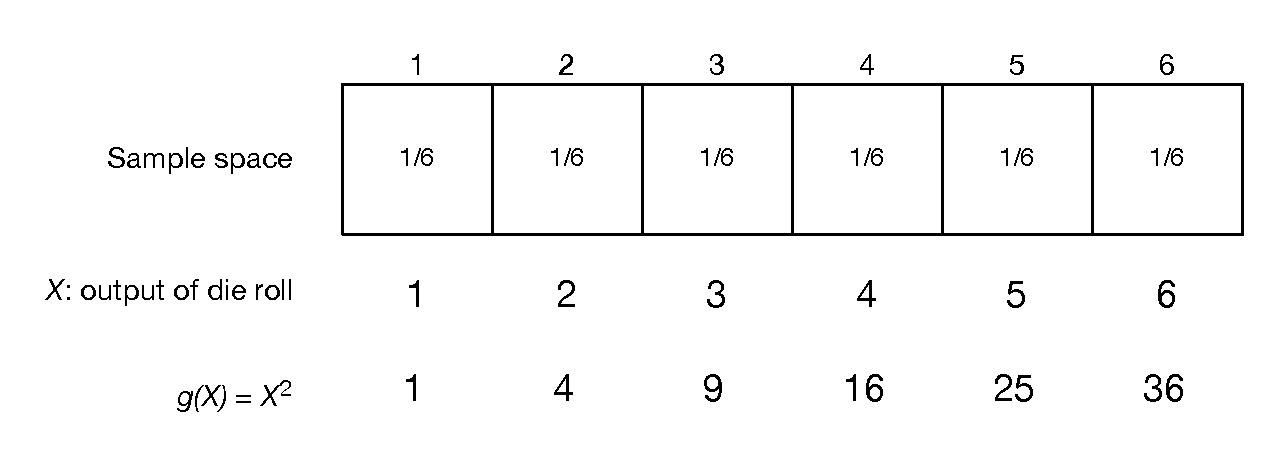
\includegraphics[width=10cm]{1diesquared}
\end{figure}
There are multiple ways to write the pmf for $g(X)$ in a table. I think the most useful way is to take the pmf table for $X$ and add an extra column for $g(X)$. We will see why this makes sense shortly.
\begin{figure}[H]
\centering
\begin{tabular}{l@{\hskip 2cm}l@{\hskip 2cm}l}
\toprule
$x$ & $g(x)$ & $p(x)$\\
\midrule
1 & 1 & 1/6\\
2 & 4 & 1/6\\
3 & 9 & 1/6\\
4 & 16 & 1/6\\
5 & 25 & 1/6\\
6 & 36 & 1/6\\
\bottomrule
\end{tabular}
\end{figure}

\end{example}

The expected value of a function of discrete random variable is computed in a similar fashion to the expected value of a random variable.

\begin{framed}
  \emph{Expected value of a function of a discrete random variable}\\
  \rule{\dimexpr\linewidth-2\fboxsep-2\fboxrule}{.1pt} \\
Let $Y$ be a discrete random variable with probability function $p(y)$, and let $g$ be a real-valued function. Then the expected value of the random variable $g(Y)$ is given by:
\[
\E[g(Y)] = \sum_{\text{all }y}g(y)\:p(y)
\]
where the sum is taken over all possible values $y$ can take. Note that the \emph{only} difference from the expected value of $Y$ is that we have $g(y)$ in place of $y$ in the sum. The probabilties $p(y)$ are \emph{unchanged}. This is again a weighted average, but this time we are taking a weighted average of the possible values of $g(Y)$.
\end{framed}

\begin{example}Let $X$ be the output of a standard six-sided die, and let $g(x) = x^2$. Find $E[g(X)]$.\\

We can use the formula for the expected value of a function of a random variable, together with the pmf table above to get:
\begin{align*}
\E[g(X)] &= \sum_{\text{all }x}g(x)\:p(x) \\
&= 1 \cdot \frac{1}{6} + 4 \cdot \frac{1}{6} + 9\cdot \frac{1}{6} + 16\cdot \frac{1}{6}+25\cdot \frac{1}{6}+36\cdot \frac{1}{6}\\
&= \frac{1}{6}(1 + 4 + 9 + 16 + 25 + 36)\\
&= \frac{91}{6} \approx 15.17
\end{align*}
\end{example}

Before we go on, we mention one more property of expected value: the expected value of a constant.

\begin{framed}
  \emph{Expected value of a constant}\\
  \rule{\dimexpr\linewidth-2\fboxsep-2\fboxrule}{.1pt} \\
Let $c$ be a constant. Then $\E(c) = c$. In other words, the expected value of a constant is just the constant itself.
\end{framed}

Combining this with the linearity of expectation, we get the following expression for the expected value of a shifted and scaled random variable.
\begin{framed}
  \emph{Expected value of $aY + b$}\\
  \rule{\dimexpr\linewidth-2\fboxsep-2\fboxrule}{.1pt} \\
If $Y$ is a random variable, and $a$ and $b$ are constants, then
\[
\E(aY + b) = a\E(Y) + b
\]
\end{framed}

\subsection{Variance}

So far we have seen one quantititive descriptor of the distribution of a random variable: the expected value. In this section, we discuss another descriptor: the variance. To begin, let's compare the pmfs of two discrete random variables.

\begin{example}Let $X$ be the number of heads observed when a fair coin is flipped 6 times, and let $Y$ be the uniform distribution on the integers $\{0, 1, 2, 3, 4, 5, 6\}$. Since $Y$ is the uniform distribution on a finite set with 7 elements, $\P(Y = y) = 1/7$ for all $Y$. $X$ takes the same values as $Y$ since the number of heads observed in 6 coin flips is an integer between 0 and 6. What is $\P(X = x)$? Since there are two possibilities for each flip, there are $2^6$ possible flip-sequences. The number of flip-sequences which give us $x$ heads is given by the binomial coefficient $\binom{6}{x}$ (why is this true?). Thus we have:
\[
\P(X = x) = \frac{\binom{6}{x}}{2^6}
\]
\end{example}
Putting both pmfs in tables we get:

\begin{figure}[H]
\centering
\begin{tabular}{l@{\hskip 2cm}l}
\toprule
$x$ & $p(x)$\\
\midrule
0 & 1/64\\
1 & 6/64\\
2 & 15/64\\
3 & 20/64\\
4 & 15/64\\
5 & 6/64\\
6 & 1/64\\
\bottomrule
\end{tabular}
\end{figure}

\begin{figure}[H]
\centering
\begin{tabular}{l@{\hskip 2cm}l}
\toprule
$y$ & $p(y)$\\
\midrule
0 & 1/7\\
1 & 1/7\\
2 & 1/7\\
3 & 1/7\\
4 & 1/7\\
5 & 1/7\\
6 & 1/7\\
\bottomrule
\end{tabular}
\end{figure}

Now let's look at the pmfs as histograms:
\begin{figure}[H]
\centering
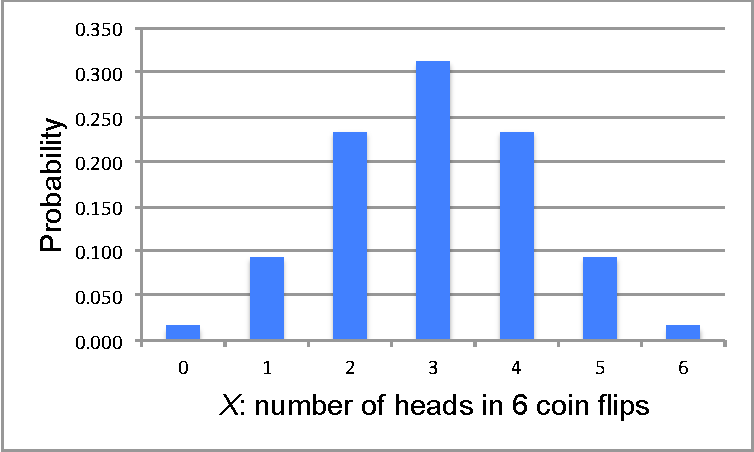
\includegraphics[width=7cm]{excelx.pdf}
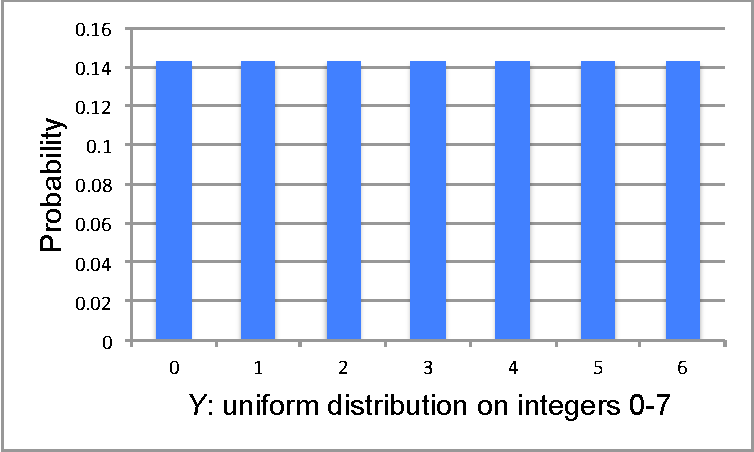
\includegraphics[width=7cm]{excely.pdf}
\end{figure}

Both of these two random variables have an expected value (mean) of 3. (You can compute it yourself if you want, or reason that both distributions are symmetric, and the ``middle'' is 3.) Despite having the same mean, the two distributions are very different. $X$ is relatively centered about the mean, while $Y$ is all ``spread out''. We want a way to quantify this amount of ``spread''. There are many ways to do this. For example, we could use the average distance from the mean. Statisticians have settled on a slightly different measure of ``spread'': the variance. In words, the variance of a random variable is the expected value of the squared-difference from the mean. Mathematically, we have the following definition:

\begin{framed}
  \emph{Variance of a discrete random variable}\\
  \rule{\dimexpr\linewidth-2\fboxsep-2\fboxrule}{.1pt} \\
Let $Y$ be a discrete random variable with probability function $p(y)$, and let $\mu = \E(Y)$ be its expected value (mean). Then we define the \emph{variance} of $Y$ by
\[
Var(Y) = \E[ (Y - \mu)^2 ]
\]
Using the formula for the expected value of a function of a random variable, this becomes
\[
Var(Y) = \sum_{\text{all }y}(y - \mu)^2 \:p(y)
\]
The variance is sometimes denoted by the symbol $\sigma^2$. The \emph{standard deviation} of a random variable is the square root of the variance, and is denoted $\sigma$.
\end{framed}

Let's compute the variance of the two random variables above. Since $Y$ is more ``spread out'' than $X$, we expect it to have a higher variance.

\begin{example}Let $X$ be the number of heads observed when a fair coin is flipped 6 times, and let $Y$ be the uniform distribution on the integers $\{0, 1, 2, 3, 4, 5, 6\}$. Compute the variances of both random variables.\\

The mean of both random variables is 3, so we have:
\begin{align*}
Var(X) &= \sum_{\text{all }x}(x - 3)^2 \:p(x) \\
&= (0-3)^2 \frac{1}{64} + (1-3)^2 \frac{6}{64} + (2-3)^2 \frac{15}{64} + (3-3)^2 \frac{20}{64} + (4-3)^2 \frac{15}{64} + (5-3)^2 \frac{6}{64} + (6-3)^2 \frac{1}{64} \\
&= \frac{(9)(1)}{64} + \frac{(4)(6)}{64} + \frac{(1)(15)}{64} + \frac{(0)(20)}{64} + \frac{(1)(15)}{64} + \frac{(4)(6)}{64} + \frac{(9)(1)}{64} \\ 
&= \frac{96}{64} \\
&= \frac{3}{2}
\end{align*}

\begin{align*}
Var(Y) &= \sum_{\text{all }y}(y - 3)^2 \:p(y) \\
&= (0-3)^2 \frac{1}{7} + (1-3)^2 \frac{1}{7} + (2-3)^2 \frac{1}{7} + (4-3)^2 \frac{1}{7} + (4-3)^2 \frac{1}{7} + (5-3)^2 \frac{1}{7} + (6-3)^2 \frac{1}{7} \\
&= \frac{1}{7}(9 + 4 + 1 + 0 + 1 + 4 + 9) \\
&= \frac{28}{7} \\
&= 4
\end{align*}
As predicted from the histograms, $Y$ has a much higher variance.
\end{example}

The variance is often not computed by using the definition above, but by using a formula affectionately known as the \emph{Magic Variance Formula}.

\begin{framed}
  \emph{Magic Variance Formula}\\
  \rule{\dimexpr\linewidth-2\fboxsep-2\fboxrule}{.1pt} \\
Let $Y$ be a random variable and let $\mu = \E(Y)$ be its expected value (mean). Then the variance of $Y$ is given by
\[
Var(Y) = \E[ Y^2 ] - \mu^2
\]
\end{framed}
To verify this formula, we expand out the binomial in the definition of variance, and use linearity of expectation.
\begin{align*}
Var(Y) &= \E[ (Y - \mu)^2] \\
&= \E( Y^2 - 2 \mu Y + \mu^2 ) \\
&= \E(Y^2) - 2 \mu \E(Y) + \E(\mu^2) \\
&= \E(Y^2) - 2 \mu^2 + \mu^2 \\
&= \E(Y^2) - \mu^2
\end{align*}
where we used the fact that $\E(Y) = \mu$, and the expected value of a constant is just the constant.\\

Variance behaves much differently from expectation. Unlike expectation, it is \emph{not} linear. For a random variable $Y$, we have the following expression for the variance of $aY + b$.

\begin{framed}
  \emph{Variance of $aY + b$}\\
  \rule{\dimexpr\linewidth-2\fboxsep-2\fboxrule}{.1pt} \\
If $Y$ is a random variable, and $a$ and $b$ are constants, then
\[
Var(aY + b) = a^2 Var(Y)
\]
\end{framed}
To see this, we use the Magic Variance Formula. First we compute $\E[(aY + b)^2]$.
\begin{align*}
\E[(aY +b)^2] &= \E(a^2 Y^2 + 2 a b Y + b^2) \\
&= a^2 \E(Y^2) + 2 a b \E(Y) + b^2
\end{align*}
where we used the linearity of expectation and the fact that the expected value of a constant is the constant itself. Next, we compute $[\E(aY + b)]^2$. Once again using linearity of expectation, we get:
\begin{align*}
[\E(aY + b)]^2 &= (a\E(Y) + b)^2 \\
&= a^2 \E(Y)^2 + 2 b \E(Y) + b^2
\end{align*}
Using the Magic Variance Formula, we subtract these two to get:
\begin{align*}
Var(aY + b) &= \E[(aY +b)^2] - [\E(aY + b)]^2 \\
&= \left( a^2 \E(Y^2) + 2 a b \E(Y) + b^2 \right) - \left( a^2 \E(Y)^2 + 2 b \E(Y) + b^2 \right) \\
&= a^2 \left( E(Y^2) - [E(Y)]^2 \right) \\
&= a^2 Var(Y)
\end{align*}
where in the final line we have used the Magic Variance Formula one final time. \\

Note that the $b$ disappears entirely. Why does this make sense? The variance represents the spread of a random variable around its mean. Shifting a random variable by a constant amount should not affect this spread.\\

We conclude this section with a result about the variance of a sum of \emph{independent} random variables which we will need later. We have not formally defined independence for random variables, but the intuition is that the output of one does not affect the output of each other. This result is only true for independent random variables.

\begin{framed}
  \emph{Variance of a sum of independent random variables}\\
  \rule{\dimexpr\linewidth-2\fboxsep-2\fboxrule}{.1pt} \\
If $X_1, X_2, \dots, X_n$ are \emph{independent} random variables, then
\[
Var(X_1 + X_2 + \cdots + X_n) = Var(X_1) + Var(X_2) + \cdots + Var(X_n)
\]
i.e. the variance of a sum is the sum of the variances. This is only true for independent random variables.
\end{framed}

\subsection{Bernoulli Trials}
One of the simplest models in probability is that of a sequence \emph{Bernoulli trials}. Essentially Bernouilli trials are the generalization of repeated coin tossing. 

\begin{framed}
  \emph{Bernouilli trials}\\
  \rule{\dimexpr\linewidth-2\fboxsep-2\fboxrule}{.1pt} \\
A sequence of Bernoulli trials is a sequence of experiements satisfying the following assumptions:
\begin{enumerate}
\item Each trial has exactly two possible outcomes, designated \emph{success} and \emph{failure}.
\item The trials are independent, i.e. the outcome of one trial does not influence the outcome of any other trial.
\item On each trial, the probability of success is $p$ and the probability of failure is $1-p$, where $0 \leq p \leq 1$. (Sometimes, for convenience, we define $q = 1 - p$).
\item These probabilities are constant for all trials, i.e. $p$ does not change as the experiment is repeated.
\end{enumerate}
\end{framed}

Since Bernoulli trials have only two possible outcomes, we can think of them as ``yes or no'' events. Here are some examples of Bernoulli trials:
\begin{enumerate}
\item Flipping a coin of a coin, where we designate a flip of heads as a success. If it is a fair coin, then $p = 1/2$. If it is an unfair coin, then $p \neq 1/2$. 
\item Rolling two standard, six-sided dice, where we designate a roll of doubles as success (and every other roll is failure). This is how you roll to get out of jail in Monopoly.
\item Playing a slot machine in Las Vegas.
\item Calling a registered voter uniformly at random and asking them if they are voting for Hillary Clinton.
\item Repeated free throw attempts by your instructor, assuming that he never improves.
\end{enumerate}

Here are some examples of trials which are not Bernouilli trials. Why are these not Bernouilli trials?
\begin{enumerate}
\item Drawing cards one at a time from a standard deck of 52 playing cards, where we designate success as drawing an ace.
\item Calling a list of 100 registered voters one-at-a-time and asking them if they are voting for Hillary Clinton.
\item Repeated free throw attempts by your instructor, assuming his skill can improve (if only a little) with practice.
\end{enumerate}

An individual Bernoulli trial modeled by a Bernoulli random variable.

\begin{framed}
  \emph{Bernoulli random variable}\\
  \rule{\dimexpr\linewidth-2\fboxsep-2\fboxrule}{.1pt} \\
A \emph{Bernoulli random variable} $Y$ with parameter $p$ is a random variable which is 1 with probability $p$ and 0 with probability $1 - p$. It models a single Bernoulli trial, where 1 indicates success and 0 indicates failure. We can write its pmf in the table below:
\begin{figure}[H]
\centering
\begin{tabular}{l@{\hskip 2cm}l}
\toprule
$y$ & $p(y)$\\
\midrule
0 & $1 - p$\\
1 & $p$ \\
\bottomrule
\end{tabular}
\end{figure}
To indicate that $Y$ is a Bernoulli random variable with paramater $p$, we will sometimes write $Y \sim$ Bernoulli($p$).
\end{framed}

What is the mean and variance of a Bernoulli random variable? Let $Y \sim$ Bernoulli($p$). Then for the expected value:
\begin{align*}
\E(Y) &= \sum_{\text{all }y}y\:p(y) \\
&= 0(1 - p) + 1(p) \\
&= p
\end{align*}
For the variance, we will use the Magic Variance Formula. This requires computing $\E(Y^2)$.
\begin{align*}
\E(Y^2) &= \sum_{\text{all }y}y^2\:p(y) \\
&= 0^2(1 - p) + 1^2(p) \\
&= p
\end{align*}
By the Magic Variance Formula,
\begin{align*}
Var(Y) &= \E(Y^2) - [E(Y)]^2 \\
&= p - p^2 \\
&= p(1-p)
\end{align*}
Summarizing, these results, we have:
\begin{framed}
  \emph{Characteristics of a Bernoulli random variable}\\
  \rule{\dimexpr\linewidth-2\fboxsep-2\fboxrule}{.1pt} \\
Let $Y$ be a Bernouilli random variable with parameter $p$. Then:
\begin{align*}
\E(Y) &= p \\
Var(Y) &= p(1-p) = pq
\end{align*}
where $q = 1-p$.
\end{framed}

Bernoulli trials are useful in many situations. Here are two questions we might want to ask about a sequence of Bernoulli trials.

\begin{enumerate}
\item How many successes do we have out of a \emph{fixed} number of trials?
\item How many trials does it take to get our first success?
\end{enumerate}

The first question is answered by the binomial distribution, and the second by the geometric distribution.

\subsection{Binomial distribution}

The binomial distribution models the number of successes in a fixed number of Bernoulli trials. Let's start with an example.

\begin{example}Suppose we are playing a slot machine in Las Vegas. Suppose $p$ is the probabiltiy of winning on one play\footnote{This can be quite different depending on the type of slot machine you are playing, although all slot machines are designed so that you lose money on average. There are numerous websites devoted to slot machine odds.}. Suppose you play 10 times. What is the probability that you win 2 times?\\

First, this is an example of Bernoulli trials, since each play of the slot machine has two possible outcomes (win and loss), is independent, and the probability of winning is does not change as you continue to play. \\

What is the sample space for this problem? Let us use the symbol \texttt{W} for a win and the symbol \texttt{L} for a loss. Then any sequence of 10 plays can be represented as a sequence of 10 \texttt{W}s and \texttt{L}s. One sequence might be \texttt{LLWLLWLLLL}. Is each sequence equally likely? Unless $p = 1/2$, different sequences can have different probabilities. For example, if $p < 1/2$, \texttt{LLLLLLLLLL} is much more probable than \texttt{WWWWWWWWWW}. What is the probability of a given sequence? Since we are looking at the probability of 2 wins (and thus 8 losses), let's look at a typical sequence where this is the case: \texttt{LLWLLWLLLL}. Since these are Bernoulli trials and thus each trial is independent, we just multiply together the probability of winning or losing at each trial.
\[
\P(\texttt{LLWLLWLLLL}) = (1-p)(1-p)p(1-p)(1-p)p(1-p)(1-p)(1-p)(1-p) = p^2(1-p)^8
\]
We see from this that the probability of a sequence depends only on the total number of wins and losses, not on the order in which those wins and losses occur. Thus the probability of \emph{any} sequence of 10 trials composed of 2 wins and 8 losses will be $p^2(1-p)^8$.\\

The only question remaining is how many events in the sample space correspond to 2 wins and 8 losses, i.e. how many strings of length 10 contain exactly 2\texttt{W}s and 8\texttt{L}s? Recalling our combinatorics, this is given by the binomial coefficient $\binom{10}{2}$. Since each such string is a simple event in our sample space, we add up the probabilities of all $\binom{10}{2}$ of them to get:
\[
\P(\text{2 wins out of 10 trials})= \binom{10}{2} p^2 (1-p)^8
\]  
\end{example}

We now generalize this. Suppose we have a sequence of $n$ Bernoulli trials, with probability of success $p$ for each trial. What is the probability of obtaining $y$ successes, where $y$ is an integer between 0 and $n$? If we designate success by \texttt{S} and failure by \texttt{F}, we can take the sample space to be strings of $n$ letters, where each letter is either \texttt{S} or \texttt{F}. Just as in the example above, the probability of any string depends only on the number of \texttt{S}s and \texttt{F}s, not on their order. If we have $y$ successes, this corresponds to a string of length $n$ with $y$ \texttt{S}s and $(n-y)$ \texttt{F}s. The probability of that event is $p^y(1-p)^{n-y}$. Using the binomial coefficient, the number of strings of length $n$ composed of $y$ \texttt{S}s and $(n-y)$ \texttt{F}s is $\binom{n}{y}$. Thus we have:
\[
\P(\text{$y$ successes out of $n$ trials})= \binom{n}{y} p^y (1-p)^{n-y}
\]

This probability distribution, which repesents the number of successes in a fixed number $n$ Bernouilli trials, is called the \emph{binomial probability distribution}. A random variable $Y$ with this distribution is called a \emph{binomial random variable}.

\begin{framed}
  \emph{Binomial distribution}\\
  \rule{\dimexpr\linewidth-2\fboxsep-2\fboxrule}{.1pt} \\
A discrete random variable $Y$ has a \emph{binomial distribution} with $n$ trials and probability of success $p$ if
\begin{align*}
p(y) &= \binom{n}{y} p^y (1-p)^{n-y} & y = 0, 1, \dots, n
\end{align*}
$Y$ is a \emph{binomial random variable} with parameters $n$ and $p$, written $Y \sim \text{Binomial}(n, p)$. This models the number of successes out of $n$ Bernoulli trials, where the probability of a single success is $p$.
\end{framed}

First let's check to make sure $Y$ is a well-defined discrete random variable, i.e. the probabilities of all its possible outputs sum to 1. Using the binomial theorem, we see that
\begin{align*}
\sum_{y=0}^n p(y) = \sum_{y=0}^n \binom{n}{y} p^y (1-p)^{n-y} = \left[p + (1 - p)\right]^n = 1^n = 1
\end{align*}

What is the expected value and variance of a binomial random variable? There are many ways to compute this, but we will use a clever trick based on linearity. Let $Y \sim \text{Binomial}(n, p)$. For each trial $i = 1, 2, \dots, n$ let:
\[
Y_i = \begin{cases}
0 & \text{trial $i$ is a failure}\\
1 & \text{trial $i$ is a success}
\end{cases}
\]
Since $\P(Y_i = 1) = p$, $Y_i \sim \text{Bernoulli}(p)$. Since each Bernoulli random variable is 1 only if that trial is a success and $Y$ is the number of trials,
\[
Y = Y_1 + Y_2 + \cdots + Y_n
\]
Using the linearity of expectation, 
\begin{align*}
\E(Y) &= \E(Y_1 + Y_2 + \cdots + Y_n) \\
&= \E(Y_1) + \E(Y_2) + \cdots + \E(Y_n) \\
&= p + p + \cdots + p = np
\end{align*}
Furthermore, since Bernoulli trials are independent, the $Y_i$ are all independent. Thus we can do the same thing for the variance:
\begin{align*}
Var(Y) &= Var(Y_1 + Y_2 + \cdots + Y_n) \\
&= Var(Y_1) + Var(Y_2) + \cdots + Var(Y_n) \\
&= p(1-p) + p(1-p) + \cdots + p(1-p) = np(1-p)
\end{align*}

Summarizing these properties, we have:

\begin{framed}
\emph{Properties of binomial distribution}\\
  \rule{\dimexpr\linewidth-2\fboxsep-2\fboxrule}{.1pt} \\
Let $Y$ be a binomial random variable with parameters $n$ and $p$. Then
\begin{align*}
\E(Y) &= np \\
Var(Y) &= np(1-p)
\end{align*}
\end{framed}

Let's look at histograms of the binomial distribution for a few choices of parameters. First here are histograms for $p=1/2$ (fair coin):
\begin{figure}[H]
\centering
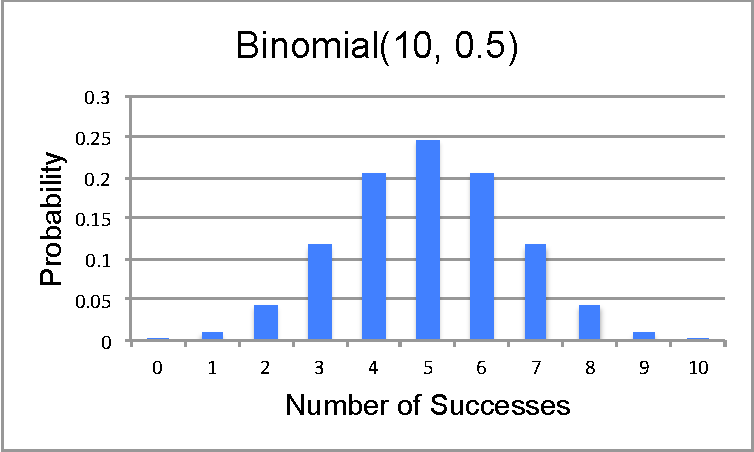
\includegraphics[width=8cm]{binomial105}
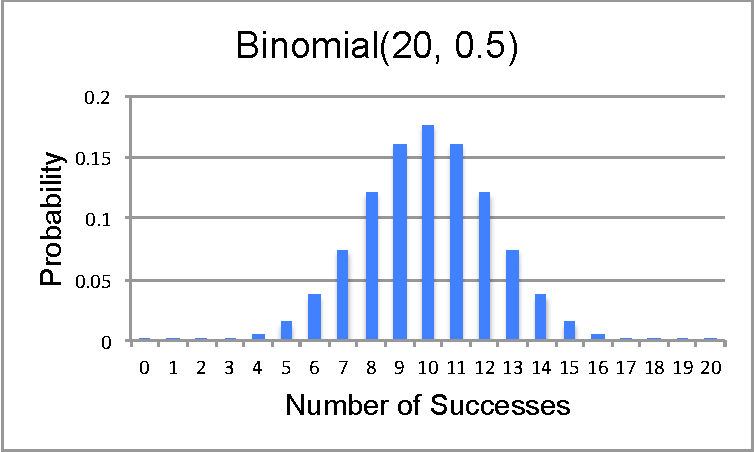
\includegraphics[width=8cm]{binomial205}
\end{figure}
These distributions are perfectly symmetric about the mean, which is expected for the case where $p = 1/2$. Note that as $n$ increases, these look more and more like ``bell curves''. While we have not yet talked about the normal distribution, keep in mind how these histograms look. For large enough $n$, we will be able to approximate the (discrete) binomial distribution by the (continuous) normal distribution.\\

The histograms look a bit different for $p$ significantly different from 1/2. These histograms are for $p = 0.2$.
\begin{figure}[H]
\centering
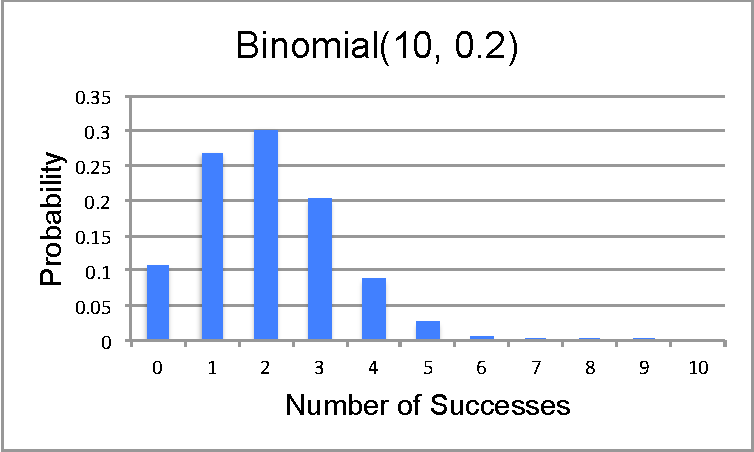
\includegraphics[width=8cm]{binomial102}
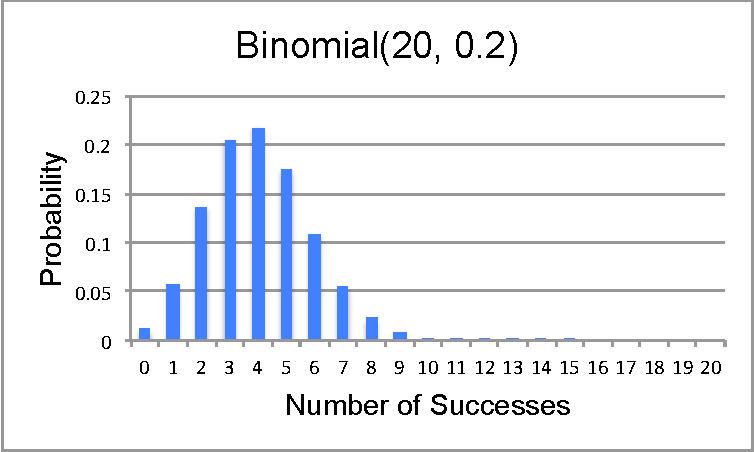
\includegraphics[width=8cm]{binomial202}
\end{figure}

These are not symmetric. Since $p < 1/2$, the distributions are skewed to the left, which is what we expect since failure is more likely that success. Although not to the same extent as the case where $p = 1/2$, these also start to look like bell curves as $n$ increases. We will also be able to approximate these by normal distributions for large $n$, but the farther $p$ is from 1/2, the larger $n$ will need to be for this approximation to be reasonable.

\begin{example}When a certain variety of pea plant with purple flowers is cross-fertilized, the offspring have purple flowers 3/4 of the time and white flowers 1/4 of the time\footnote{This is one of the varieties Gregor Mendel tested. In this problem, the pea plants are heterozygous for flower color, i.e. genotype Pp.}. 
\begin{enumerate}
\item You cross-fertilize 20 of these pea plants. What is the the probability that none of them are white?\\

We can model this problem as a sequence of 20 Bernoulli trials, with ``success'' defined as a cross-fertilization producing a white flower. (Are all the assumptions of Bernouilli trials satisfied here?) Since we are looking for the number of successes in a \emph{fixed} number of trials, this is a binomial distribution. Let $X \sim Binomial(20, 1/4)$. Then, using the binomial pmf:
\[
\P(X = 0) = \binom{20}{0}\left(\frac{1}{4}\right)^0 \left(\frac{3}{4}\right)^{20} = \left(\frac{3}{4}\right)^{20} \approx 0.0032
\]
In other words, it is highly unlikely that we will have no white flowers.

\item What is the probability that we will have at least 2 white flowers?\\

Let $A$ be the event that we get at least two white flowers. It is much easier here to compute the probability of the opposite event $A^c$, the event that we get 0 or 1 white flower. 
\begin{align*}
\P(A^c) &= \P(X = 0) + \P(X = 1) \\
&= \binom{20}{0}\left(\frac{1}{4}\right)^0 \left(\frac{3}{4}\right)^{20} + \binom{20}{1}\left(\frac{1}{4}\right)^1 \left(\frac{3}{4}\right)^{19} \\
&= \left(\frac{3}{4}\right)^{20} + 20 \left(\frac{1}{4}\right) \left(\frac{3}{4}\right)^{19} \approx 0.024
\end{align*}
Thus we have $\P(A) = 1 - \P(A^c) = 0.976$.

\item What is the expected number of white flowers? \\

The expected value of a binomial random variable is $np$. For this case, we have $n = 20$ and $p = 0.25$, thus
\[
\E(X) = n p = (20)(0.25) = 5
\]
\end{enumerate} 
\end{example}

% end of class 5
\end{document}

\subsection{Geometric Distribution}

The geometric distribution models the number of Bernoulli trials it takes to get the first success. Using the slot machine example from the previous section, if were willing to play a slot machine repeatedly until you won (i.e. you had infinite patience and money), the number of plays it took to get your first win would follow the geometric distribution.\\

Consider a sequence of Bernoulli trials with probability of success $p$. Here is our experiment: we will perform a series of trials until we get a success. The outcome of the experiment is the number of trials it takes to get our first success. Let $Y$ be the random variable denoting the number of the trial on which the first success occurs.
The smallest possible value for $Y$ is 1, since we could succeed the first time\footnote{$Y$ cannot be 0, since you cannot succeed if you don't play.}. However, there is no upper limit for $Y$; in principle, the trials could go on indefinitely. $Y$ is a discrete random variable, but $Y$ can take values in the countably infinite set $\N = 1, 2, 3, \dots$. This is the first example we have seen of a discrete random variable with a countable range.\\

As in the binomial case, we can describe all possible outputs of our experiment by strings consisting of the letters \texttt{S} and \texttt{F}, where \texttt{S} indicates a success and \texttt{F} indicates a failure. This time, however, the strings are not of fixed length; however, the final element in each string is always \texttt{S}, and every element before that is \texttt{F}. The event $(Y = 1)$ corresponds to the string \texttt{S}, $(Y = 1)$ corresponds to \texttt{FS}, etc. Since the trials are independent, we have the following table for the pmf of $Y$.

\begin{figure}[H]
\centering
\begin{tabular}{llll}
\toprule
$y$ & event && $p(y)$\\
\midrule
1 & \texttt{S}     & success on first trial                          & $p$\\
2 & \texttt{FS}    & failure on first trial, success on second trial & $(1-p)p$\\
3 & \texttt{FFS}   & first success on third trial                    & $(1-p)^2 p$\\
4 & \texttt{FFFS}  & first success on fourth trial                   & $(1-p)^3 p$\\
& \vdots & & \vdots \\
$k$ & $\underbrace{ \texttt{FFF}\dots\texttt{F}}_{\text{$k - 1$ times}}$\texttt{S} & first success on $k$th trial & $(1-p)^{k-1} p$ \\
& \vdots & & \vdots \\
\bottomrule
\end{tabular}
\end{figure}

We use this pmf to define a geometric random variable.

\begin{framed}
  \emph{Geometric distribution}\\
  \rule{\dimexpr\linewidth-2\fboxsep-2\fboxrule}{.1pt} \\
A discrete random variable $Y$ has a \emph{geometric distribution} with probability of success $p$ if: 
\begin{align*}
p(y) &= (1-p)^{y-1} p & y = 1, 2, 3, \dots
\end{align*}
$Y$ is a \emph{geometric random variable} with parameter $p$, written $Y \sim \text{Geometric}(p)$. This models the number of trials it takes to get the first success, where the probability of a single success is $p$.
\end{framed}

Here are histograms for the geometric distribution for parameters 0.5 and 0.2. 

\begin{figure}[H]
\centering
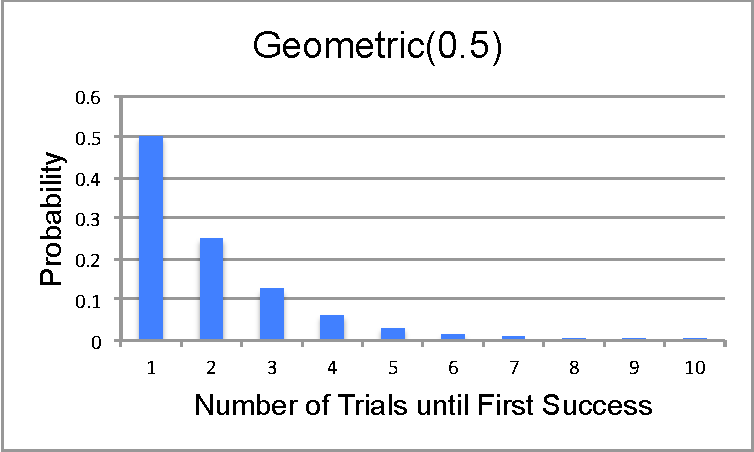
\includegraphics[width=8cm]{geometric5}
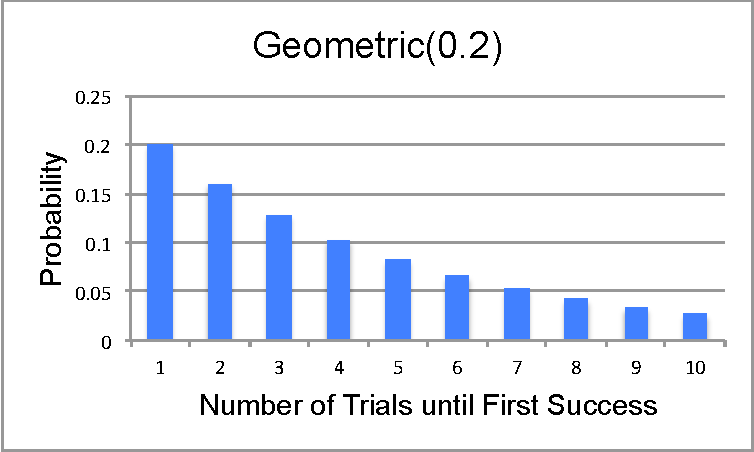
\includegraphics[width=8cm]{geometric2}
\end{figure}

Note that in all cases, the probability $p(y)$ decreases as $y$ increases. Why does this make sense? The decrease is less prominent for the $p = 0.2$ case since failure is more likely; thus it should take a greater number of trials to get a single success.\\

Just as in the case for a binomial random variable, we will verify that a geometric random variable is a valid random variable by proving that the probabilities of all its possible outputs sum to 1. We will also find its expected value and variance.\\

Before we do that, we need a result about the sum of a geometric series. This may be familiar from precalculus or calculus. There are many ways to state this result. This is the one that I like.

\begin{framed}
  \emph{Geometric series}\\
  \rule{\dimexpr\linewidth-2\fboxsep-2\fboxrule}{.1pt} \\
A \emph{geometric series} is a series whose successive terms are related by a common ratio. We can write a generic geometric series as:
\[
a + ar + ar^2 + ar^3 + \cdots = \sum_{k=1}^{\infty} ar^{k-1}
\]
In this case, the first term is $a$ and the common ratio is $r$. If $\abs{r} < 1$, then the infinite series converges, and:
\[
\sum_{k=1}^{\infty} ar^{k-1} = \frac{a}{1-r}
\]
\end{framed}

Let's use this result to show that the probabilties of a geometric random variable sum to 1. Let $Y$ be a geometric random variable with parameter $p$. Then
\begin{align*}
\sum_{y=1}^{\infty} p(y) &= \sum_{y=1}^{\infty} p (1-p)^{k-1}\\
&= \frac{p}{1 - (1 - p)} \\
&= \frac{p}{p} \\
&= 1
\end{align*}
where we used the formula above with the first term $a = p$ and the common ratio $r = p-1$.

For the expected value and variance of a geomtric random variable we have the following.

\begin{framed}
\emph{Properties of geometric distribution}\\
  \rule{\dimexpr\linewidth-2\fboxsep-2\fboxrule}{.1pt} \\
Let $Y$ be a geometric random variable with parameter $p$. Then
\begin{align*}
\E(Y) &= \frac{1}{p} \\
Var(Y) &= \frac{1-p}{p^2}
\end{align*}
\end{framed}
The variance is tedious to prove, and since not much is gained by doing it, we will omit it. The proof of the expected value involves a nice calculus trick. We will assume that $p$ is between 0 and 1, since if $p$ = 1, you are guaranteed to get your first success on the first trial, and if $p = 0$, you can never succeed.
\begin{align*}
\E(Y) &= \sum_{y=1}^{\infty} y p(y) &\text{definition of expected value} \\
&= \sum_{y=1}^{\infty} y (1-p)^{y-1} p \\
&= p \sum_{y=1}^{\infty} y q^{y-1} &\text{writing $q = 1-p$, for convenience}\\
&= p \sum_{y=1}^{\infty} \frac{d}{dq}q^y &\text{power rule of differentiation}\\
&= p \frac{d}{dq} \sum_{y=1}^{\infty} q^y &\text{swapping summation and differentiation}\footnote{This can be justified; if you want to know more about this and/or find these types of mathematical subtleties interesting, I recommend taking a course in real analysis.}\\
&= p \frac{d}{dq}\left(\frac{q}{1-q}\right) & \text{geometric series; first term $q$, common ratio $q < 1$}\\
&= p \frac{(1-q)(1) - (q)(-1)}{(1-q)^2} & \text{quotient rule of differentiation} \\
&= \frac{p}{p^2} \\
&= \frac{1}{p} 
\end{align*}

The geometric distribution is often used the model the distribution of how long you need to wait for a particular event to happen. In this case, the waiting time is given in discrete ``chunks'' of time such as hours or days.

\begin{example}You are using a computer which runs Windows 10\footnote{This problem is not intended to be an endorsement of any particular operating system.}. Suppose the probability of Windows 10 crashing in any given 1-hour period is 0.05. 

\begin{enumerate}
\item What is the probability that the computer crashes within the first two hours after you start it up?

Measuring time in one-hour intervals, let $X$ be the number of one-hour intervals until your computer crashes. We will model $X$ as a geometric random variable with parameter $p = 0.05$. We are looking for $\P(X \leq 2)$:
\begin{align*}
\P(X \leq 2) &= \P(X = 1) + \P(X = 2) \\
&= p + (1-p)p \\
&= (0.05) + (0.95)(0.05) \\
&= 0.0975
\end{align*}

\item What is the probability that your computer will still be running two hours after you start it up?\\

Here want the probability that the first crash occurs after Hour 2. There are two equivalent ways to look at this. First we can compute $\P(X > 2)$ directly using the result from the first part.
\begin{align*}
\P(X > 2) &= 1 - \P(X \leq 2) \\
&= 1 - 0.0975 \\
&= 0.9025
\end{align*}
Alternatively, the probability that your computer is still running after two hours is equal the probability that it does not crash in Hour 1 and that it does not crash in Hour 2.
\begin{align*}
\P(X > 2) &= \P(\text{no crash in Hour 1} \cap \text{no crash in Hour 2} ) \\
&= \P(\text{no crash in Hour 1})\: \P(\text{no crash in Hour 2}) \\
&= (1-p)^2\\
&= 0.95^2\\
&= 0.9025
\end{align*}
There is a rougly 90\% chance your computer is still running after two hours. 

\item Given that your computer is still running at the 10-hour mark, what is the probability that it is still running after two more hours?\\

Here, we want the probability that the computer does not crash in Hour 11 or Hour 12 give than it has made it to the 10-hour mark. Since the computer has made it to the 10-hour mark, we know that $X > 10$. We are interested in $\P(X > 12 | X > 10)$. By the definition of conditional probability,
\begin{align*}
\P(X > 12 | X > 10) &= \frac{\P(X > 12 \cap X > 10)}{\P(X>10)}\\
&= \frac{\P(X > 12)}{\P(X>10)}
\end{align*}
since if $X > 12$, then it must also be true that $X > 10$. Using the same logic as in the second method of the previous part, if $X>12$, then the computer must not have crashed in Hours 1-12, so $\P(X > 12) = (1-p)^{12}$. Similarly, $\P(X > 10) = (1-p)^{10}$. Plugging these in above, we get
\begin{align*}
\P(X > 12 | X > 10) = \frac{(1-p)^{12}}{(1-p)^{10}} = (1-p)^2 = \P(X > 2) = 0.9025
\end{align*}
Thus the probability that the computer is still running after two more hours given that it has already been running for 10 hours is the same as the probabiltiy that the computer is still running two hours after startup. This property of the geometric distribution is called \emph{memorylessness}
\end{enumerate}
\end{example}

Is the geometric distribution a good model for the previous problem? The assumption here is that the probability of crashing within any one-hour period is constant, no matter how long the computer is running for. Since you are the one modeling the problem, you need to decide how reasonable this assumption is. Do you expect this to be the case, or do you, for example, expect that a particular computer will be more likely to crash the longer it has been running? This can depend on many factors including the age of the computer and the OS it is running. Perhaps it is reasonable assumption if the computer has only been running for a short period of time. \\

The memoryless property, which we observed in the previous example, is a fundamental property of the geometric distribution. We can state it mathematically in the following way.

\begin{framed}
\emph{Memoryless property of the geometric distribution}\\
  \rule{\dimexpr\linewidth-2\fboxsep-2\fboxrule}{.1pt} \\
Let $Y$ be a geometric random variable with parameter $p$. Then for all $m$ and $n$
\begin{align*}
\P(Y > m + n | Y > m) = \P(Y > n)
\end{align*}
If the first success has \emph{not} occurred by trial number $m$, the distribution of the remaining number of trials needed to get the first success is the same as if you started from scratch.
\end{framed}

If we think of Bernoulli trial in terms of a casino game such as roulette, the memoryless property of the geometric distribution makes sense. The individual spins of a roulette wheel are independent, so no betting strategy based on past outcomes of the roulette wheel can work.

\subsection{The Hypergeometric Distribution}

In this section we will look briefly at the hypergeometric distribution, which models sampling without replacement.
Consider the following example.

\begin{example}You have a bag of 20 marbles, 12 of which are red and 8 of which are black.
\begin{enumerate}
\item You draw a single marble from the bag five times, replacing it before each new draw. What is the probabiltiy that 3 of the 5 marbles drawn are red?\\

This can be modeled with a binomial random variable. Since the marbles are replaced before each draw, the probability of drawing a red marble is constant at $12/20 = 0.6$. The draws are thus independent, so we have a sequence of 5 Bernoulli trials. Considering a draw of a red marble as a success, let $X\sim\text{Binomial}(5, 0.6)$. Then:
\[
\P(X = 3) = \binom{5}{3} 0.6^3 0.4^2 \approx 0.346
\]

\item You draw five marbles from the bag without replacement. What is the probability that 3 of the 5 marbles drawn are red?\\

This time we cannot use the binomial distibution since the probability of drawing a red marble changes as marbles are drawn from the bag. Using combinatorics, there are $\binom{20}{5}$ possible draws. There are $\binom{12}{3}$ ways to choose 3 of the 12 red marbles, and $\binom{8}{2}$ ways to choose 2 of the 12 black marbles. Letting $Y$ be the number of red marbles in our sample of 5, we have
\[
\P(Y = 3) = \frac{ \binom{12}{3}\binom{8}{2}}{\binom{20}{5}} \approx 0.397
\]
\end{enumerate}
\end{example}

The probabilties here are quite different (by about 5\%). Since we are sampling 1/4 of the total marbles, it is unsurprising that there is a significant difference between sampling without replacement and sampling with replacement. What would happen if sampled a smaller fraction of the total marbles?

\begin{example}Repeat the previous problem if we instead have a bag of 200 marbles, 120 of which are red and 80 of which are black.\\

If we sample with replacement, the probability will not change; if $X$ is the number of red marbles drawn out of 5, we still have $X \sim \text{Binomial}(5, 0.6)$, so $\P(X = 3) = 0.346$. For sampling without replacement, let $Y$ again be the number of red marbles out of a sample of 5. Then
\[
\P(Y = 3) = \frac{ \binom{120}{3}\binom{80}{2}}{\binom{200}{5}} \approx 0.350
\]
\end{example}

In this case, the two probabililies differ by only about 0.5\%, which is much smaller. The take-home message here is that if we sample a fraction of the total population, sampling without replacement is approximately equivalent to sampling with replacement, i.e. we can approximate sampling without replacement by a binomial distribution.\\

The distribution for sampling without replacement in this scenario is known as the \emph{hypergeometric distribution}. It applies whenever we sample without replacement from a population which can be divided into two distinct groups. Examples of the hypergeometric distribution include:
\begin{enumerate}
\item Drawing a sample without replacement from a bag of marbles of two different colors.
\item Polling a sample of a population of eligible voters with a yes-no question or a choice between two candidates.
\item Drawing to complete a flush in Texas Hold'em poker. If, for example, the player has four clubs after the flop, then the probability of getting a club on the next two draws is hypergeometric since the draws are done without replacement.
\end{enumerate}

The pmf for the hypergeometric distribution can be derived from combinatorics. I include it here for completeness and as an application of combinatorics. You do not need to memorize it, and there will be no homework or exam problems which require the direct use of the hypergeometric pmf. That being said, you do need to know the combinatorics behind sampling without replacement and problems involving calculating probabilities for sampling without replacement, like the examples above, are fair game.\\

We will write the hypergeometric pmf in terms of the marble problem. Suppose we have a bag of $N$ marbles, $r$
of which are red and the remaining $(N - r)$ of which are black. Suppose we take a sample of $n$ marbles from the bag without replacement. Let $Y$ be the number of marbles in our sample. Then the random variable $Y$ has a hypergeometric distribution, and:
\[
\P(Y = y) = \frac{ \binom{r}{y} \binom{N-r}{n-y} }{ \binom{N}{n} }
\]
where $y = 0, 1, 2, \dots, n$. We have the additional restrictions that $y \leq r$ and $n - y \leq N - r$, which ensure we cannot draw more red or black marbles than are initially present in the bag.\\

To see this, note that there are a total of $\binom{N}{n}$ possible draws (order does not matter). The number of ways to choose $y$ red marbles out of a total of $r$ red marbles is $\binom{r}{y}$. The remaining $(n - y)$ marbles in the sample of $n$ marbles must be black, and there are $\binom{N - r}{n - y}$ ways of choosing $(n - y)$ black marbles from a total of $(N - r)$ black marbles. \\

The final question to settle is when can we approximate a hypergeometric distribution (sampling without replacement) by a binomial distribution (sampling with replacement)? There is no hard-and-fast rule, but a good guideline is that if the sample size is less than 1/20 of the population size, the binomial distribution is a reasonable approximation. 

\subsection{Poisson Distribution}

The Poisson distribution is the final discrete probability distribution we will discuss in this course. It it used to model the number of events which occur during a fixed interval of time (or space) under the following two assumptions:
\begin{enumerate}
\item The average rate of occurrence of the events is constant.
\item The events occur independently from each other.
\end{enumerate}
Often the event in question is relatively rare. Examples of situations in which a Poisson distirbution is a good model include:
\begin{enumerate}
\item The number of phone calls received per hour at a call center.
\item The number of pieces of non-junk mail received per day.
\item The number of traffic accidents occurring at a particular intersection per week.
\item The number of customers who enter a restaurant during a 15-minute period (although you might argue here that the average rate of arrival changes depending on the time of day.)
\item The number of decays per second of a radioactive isotope.
\item The number of errors per page in a manuscript.
\end{enumerate}

Let's take the first example. Let $Y$ be the number of calls received per hour at a call center, and suppose the average number of calls per hours is $\lambda$. We will do the following:
\begin{enumerate}
\item Split our hour up into $n$ subintervals, where each subinterval is so small that at most one phone call can occur per subinterval. Let $p$ be the probability that a phone call occurs in a given subinterval. 
\item We can then model $Y$ as $Y \sim \text{Binomial}(n, p)$, since the total number of calls in one hour is the total number of subintervals which contain one call.
\item The mean of $Y$ is $np$, since it is a binomial random variable. Since the average number of calls per hour is $\lambda$, we will let $\lambda = np$ so $p = \lambda / n$
\item According to the binomial distribution, the probability $p(y) = \P(Y = y)$ is:
\begin{align*}
p(y) = \binom{n}{y} p^y(1-p)^{n-y} = \frac{n!}{y!(n-y)!}\left(\frac{\lambda}{n}\right)^y\left(1 - \frac{\lambda}{n}\right)^{n-y}
\end{align*}
\item Finally, we will let $n \rightarrow \infty$.
\begin{align*}
\lim_{n \rightarrow \infty} p(y) &= \lim_{n \rightarrow \infty} \frac{n!}{y!(n-y)!}\left(\frac{\lambda}{n}\right)^y\left(1 - \frac{\lambda}{n}\right)^{n-y}\\
&= \lim_{n \rightarrow \infty} \frac{n(n-1)(n-2)\cdots(n - y + 1 )}{n^y}\frac{\lambda^y}{y!}\left(1 - \frac{\lambda}{n}\right)^n \left(1 - \frac{\lambda}{n}\right)^{-y}\\
&= \frac{\lambda^y}{y!} \lim_{n \rightarrow \infty} \left(1 - \frac{\lambda}{n}\right)^n \frac{n}{n}\frac{(n-1)}{n}\frac{(n-2)}{n}\cdots\frac{(n - y + 1)}{n} \left(1 - \frac{\lambda}{n}\right)^{-y}\\
&= \frac{\lambda^y}{y!} \lim_{n \rightarrow \infty} \underbrace{\left(1 - \frac{\lambda}{n}\right)^n}_{\text{this has limit of }e^{-\lambda}} \underbrace{\left(1 - \frac{1}{n}\right)\left(1 - \frac{2}{n}\right)\cdots\left(1 - \frac{y - 1}{n}\right) \left(1 - \frac{\lambda}{n}\right)^{-y}}_{\text{these all have limit of 1}}\\
&= e^{-\lambda}\frac{\lambda^y}{y!}
\end{align*}
\end{enumerate}

The limiting probability $p(y)$ is the pmf for the \emph{Poisson distribution}.

\begin{framed}
\emph{Poisson distribution}\\
  \rule{\dimexpr\linewidth-2\fboxsep-2\fboxrule}{.1pt} \\
A discrete random variable $Y$ has a \emph{Poisson distribution} with parameter $\lambda > 0$ if 
\begin{align*}
p(y) &= e^{-\lambda}\frac{\lambda^y}{y!} &\lambda = 0, 1, 2, \dots
\end{align*}
$Y$ is called a \emph{Poisson random variable} with parameter $\lambda$, which is often denoted $Y\sim\text{Poisson}(\lambda)$.
\end{framed}
Note that the Poisson distribution can output a value of 0, which corresponds to no events happening in the fixed span of time.\\

As with the other discrete distributions, we will check that this distribution is well definied by veritying that the probabilities sum to 1.

\begin{align*}
\sum_{y=0}^\infty p(y) &= \sum_{y=0}^\infty e^{-\lambda}\frac{\lambda^y}{y!} \\
&= e^{-\lambda} \underbrace{\sum_{y=0}^\infty \frac{\lambda^y}{y!}}_{\text{Taylor series for }e^{\lambda}}\\
&= e^{-\lambda}e^{\lambda} = 1
\end{align*}

The mean of the Possion distribution is $\lambda$, which makes sense since that is the average rate of occurrence of the events which we used when we constructed the Poissin distribution as a limit of the binomial distribution. Not only is the mean of a Poisson distribution $\lambda$, but the variance is also $\lambda$. Thus we have the following properties.

\begin{framed}
\emph{Properties of the Poisson distribution}\\
  \rule{\dimexpr\linewidth-2\fboxsep-2\fboxrule}{.1pt} \\
Let $Y$ be a Poisson random variable with parameter $\lambda$. Then
\begin{align*}
\E(Y) &= \lambda \\
Var(Y) &= \lambda
\end{align*}
\end{framed}

We will prove that the mean is $\lambda$. Verifying the variance is also $\lambda$ is more tedious and will be omitted. For a Poisson random variable $Y$,

\begin{align*}
\E(Y) &= \sum_{y=0}^\infty y p(y) \\
&= \sum_{y=0}^\infty y e^{-\lambda}\frac{\lambda^y}{y!} \\
&= \sum_{y=1}^\infty e^{-\lambda}\lambda^y\frac{y}{y(y-1)!} & \text{first term of the sum is 0} \\
&= \sum_{y=1}^\infty e^{-\lambda} \frac{\lambda^y}{(y-1)!} & \text{first term of the sum is 0}
\end{align*}
Now we let $z = y - 1$. Substituting this in, we get
\begin{align*}
\E(Y) &= \sum_{y=1}^\infty e^{-\lambda} \frac{\lambda^{z+1}}{z!}\\
&= \lambda \sum_{z=0}^\infty e^{-\lambda} \frac{\lambda^{z}}{z!}\\
&= \lambda
\end{align*}
where the sum in the second-to-last line is 1 since we are summing over the entire pmf of a Poisson random variable.

\end{document}